\documentclass{article}
\usepackage[T1]{fontenc}
\usepackage[utf8]{inputenc}
\usepackage{url}
\usepackage{listings}
\usepackage{tikz}
\usepackage{float}

\lstset{
  basicstyle=\ttfamily\footnotesize,
  breaklines=true,
  breakatwhitespace=false,
  columns=fullflexible,
  keepspaces=true
}

\tikzset{
  vertex/.style={circle, draw, minimum size=8mm, inner sep=0pt},
  frontier/.style={circle, draw, fill=blue!25, minimum size=8mm, inner sep=0pt},
  visited/.style={circle, draw, fill=gray!25, minimum size=8mm, inner sep=0pt},
  undiscovered/.style={circle, draw, fill=white, minimum size=8mm, inner sep=0pt},
  treeedge/.style={very thick, blue!70!black},
  graphedge/.style={gray!70}
}

\begin{document}

\section{Introdução}
A Busca em Largura, ou \textit{Breadth-First Search} (BFS), é um dos algoritmos fundamentais de travessia em grafos \cite{cormenalgorithms}. O algoritmo parte de um vértice inicial e, em seguida, visita os demais vértices em camadas: primeiro os que estão a uma aresta de distância, depois os que estão a duas arestas, e assim sucessivamente. Dessa forma, em um grafo não ponderado, a BFS calcula a menor distância, em número de arestas, entre o vértice inicial e todos os vértices alcançáveis a partir dele. A Busca em Largura também gera uma árvore chamada \textit{Árvore de Busca em Largura}, na qual o pai de um vértice é aquele que o descobriu durante a busca.

A implementação clássica utiliza uma fila. O vértice inicial é inserido na fila, marcado como visitado, e sua distância é definida como zero. Em seguida, enquanto a fila não estiver vazia, repete-se a seguinte operação retira-se um vértice $v$ da fila e examinam-se todos os vértices $u$ vizinhos de $v$. Caso $u$ ainda não tenha sido visitado, sua distância é calculada, ele é marcado como visitado e adicionado à fila.

Uma forma simplificada do algoritmo é apresentada a seguir:

\begin{lstlisting}
BFS(G, origem):
	para cada vertice v em G:
        pai[v] = none

    pai[origem] = origem
    fila = {origem}

    enquanto fila nao esta vazia:
		u = proximo elemento da fila
		para cada vizinho v de u:
			se pai[v] == none:
				pai[v] = u
				adiciona v na fila
\end{lstlisting}


\section{BFS em Fronteiras}
O algoritmo de BFS também pode ser implementado como uma descoberta por fronteiras. Inicializa-se a primeira fronteira com o vértice inicial. Em seguida, para cada vértice presente na fronteira atual, examinam-se todos os seus vizinhos; aqueles que ainda não foram visitados são adicionados à próxima fronteira. Esse processo se repete sucessivamente, até que a fronteira atual esteja vazia.

Uma versão simplificada do algoritmo é apresentada a seguir:

\begin{lstlisting}
BFS(G, origem):
    para cada vertice v em G:
        pai[v] = none

    pai[origem] = origem
    fronteira = {origem}

    enquanto fronteira nao esta vazia:
        proxima_fronteira = vazia
        para cada vertice u na fronteira:
            para cada vizinho v de u:
                se pai[v] == none:
                    pai[v] = u
                    adiciona v na proxima_fronteira
        fronteira = proxima_fronteira
\end{lstlisting}

\subsection{Exemplo Visual de Fronteiras}

Considere o grafo da Figura~\ref{fig:bfs-step0}. A busca comeca no vertice
\texttt{A}. Em cada passo, os vertices em azul representam a fronteira atual,
os vertices em cinza ja foram visitados em niveis anteriores, e os vertices em
branco ainda nao foram descobertos. As arestas destacadas em azul formam a
arvore de BFS construida ate aquele momento. Essa arvore registra, para cada
vertice descoberto, qual foi o vertice responsavel por sua primeira descoberta.
Assim, cada aresta azul liga um vertice ao seu pai na busca, permitindo recuperar
um caminho minimo, em numero de arestas, da origem \texttt{A} ate qualquer
vertice alcancavel.

\begin{figure}[H]
\centering
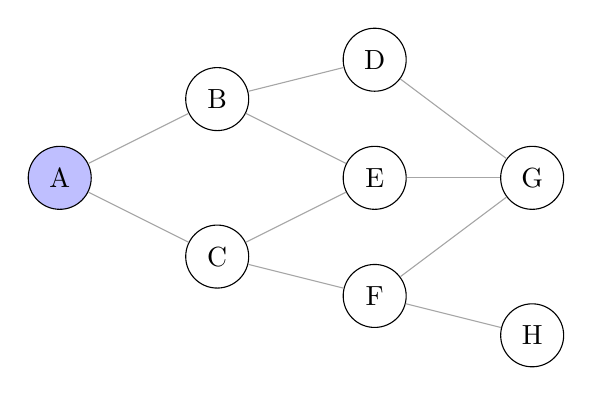
\begin{tikzpicture}[scale=1.0]
  \node[frontier] (A) at (0,0) {A};
  \node[undiscovered] (B) at (2,1) {B};
  \node[undiscovered] (C) at (2,-1) {C};
  \node[undiscovered] (D) at (4,1.5) {D};
  \node[undiscovered] (E) at (4,0) {E};
  \node[undiscovered] (F) at (4,-1.5) {F};
  \node[undiscovered] (G) at (6,0) {G};
  \node[undiscovered] (H) at (6,-2) {H};

  \draw[graphedge] (A) -- (B);
  \draw[graphedge] (A) -- (C);
  \draw[graphedge] (B) -- (D);
  \draw[graphedge] (B) -- (E);
  \draw[graphedge] (C) -- (E);
  \draw[graphedge] (C) -- (F);
  \draw[graphedge] (D) -- (G);
  \draw[graphedge] (E) -- (G);
  \draw[graphedge] (F) -- (G);
  \draw[graphedge] (F) -- (H);
\end{tikzpicture}
\caption{Passo 0 da BFS: a fronteira inicial contem apenas a origem \texttt{A}.}
\label{fig:bfs-step0}
\end{figure}

No passo inicial, a distancia de \texttt{A} e zero. A primeira expansao examina
as arestas que saem de \texttt{A}. Como \texttt{B} e \texttt{C} ainda nao foram
visitados, ambos sao descobertos, recebem distancia um e passam a formar a
proxima fronteira.

\begin{figure}[H]
\centering
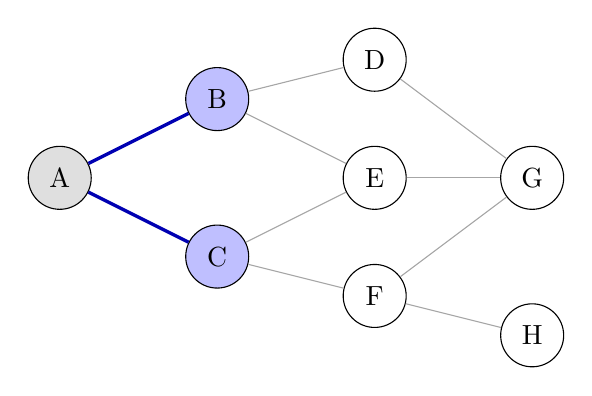
\begin{tikzpicture}[scale=1.0]
  \node[visited] (A) at (0,0) {A};
  \node[frontier] (B) at (2,1) {B};
  \node[frontier] (C) at (2,-1) {C};
  \node[undiscovered] (D) at (4,1.5) {D};
  \node[undiscovered] (E) at (4,0) {E};
  \node[undiscovered] (F) at (4,-1.5) {F};
  \node[undiscovered] (G) at (6,0) {G};
  \node[undiscovered] (H) at (6,-2) {H};

  \draw[treeedge] (A) -- (B);
  \draw[treeedge] (A) -- (C);
  \draw[graphedge] (B) -- (D);
  \draw[graphedge] (B) -- (E);
  \draw[graphedge] (C) -- (E);
  \draw[graphedge] (C) -- (F);
  \draw[graphedge] (D) -- (G);
  \draw[graphedge] (E) -- (G);
  \draw[graphedge] (F) -- (G);
  \draw[graphedge] (F) -- (H);
\end{tikzpicture}
\caption{Passo 1 da BFS: \texttt{B} e \texttt{C} formam a fronteira de nivel 1.}
\label{fig:bfs-step1}
\end{figure}

No segundo passo, a BFS expande todos os vertices da fronteira atual. O vertice
\texttt{B} descobre \texttt{D} e \texttt{E}. O vertice \texttt{C} tambem possui
uma aresta para \texttt{E}, mas \texttt{E} ja pode ter sido descoberto por
\texttt{B}; nesse caso, a implementacao mantem apenas um pai para \texttt{E}.
O vertice \texttt{C} tambem descobre \texttt{F}. Assim, a nova fronteira passa a
ser formada por \texttt{D}, \texttt{E} e \texttt{F}, todos com distancia dois.

\begin{figure}[H]
\centering
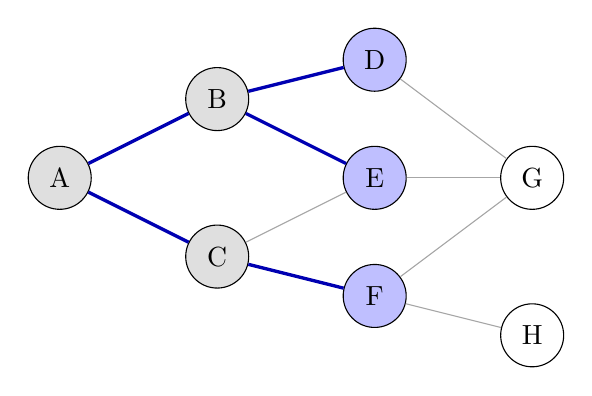
\begin{tikzpicture}[scale=1.0]
  \node[visited] (A) at (0,0) {A};
  \node[visited] (B) at (2,1) {B};
  \node[visited] (C) at (2,-1) {C};
  \node[frontier] (D) at (4,1.5) {D};
  \node[frontier] (E) at (4,0) {E};
  \node[frontier] (F) at (4,-1.5) {F};
  \node[undiscovered] (G) at (6,0) {G};
  \node[undiscovered] (H) at (6,-2) {H};

  \draw[treeedge] (A) -- (B);
  \draw[treeedge] (A) -- (C);
  \draw[treeedge] (B) -- (D);
  \draw[treeedge] (B) -- (E);
  \draw[graphedge] (C) -- (E);
  \draw[treeedge] (C) -- (F);
  \draw[graphedge] (D) -- (G);
  \draw[graphedge] (E) -- (G);
  \draw[graphedge] (F) -- (G);
  \draw[graphedge] (F) -- (H);
\end{tikzpicture}
\caption{Passo 2 da BFS: \texttt{D}, \texttt{E} e \texttt{F} formam a fronteira de nivel 2.}
\label{fig:bfs-step2}
\end{figure}

No terceiro passo, a fronteira de nivel dois e expandida. Os vertices
\texttt{D}, \texttt{E} e \texttt{F} possuem arestas para \texttt{G}. O primeiro
que conseguir registrar \texttt{G} como descoberto define seu pai na arvore de
BFS. Na figura, \texttt{E} foi escolhido como pai de \texttt{G}, mas
\texttt{D} ou \texttt{F} tambem poderiam ser pais validos, pois todos pertencem
ao nivel anterior. Alem disso, \texttt{F} descobre \texttt{H}, que tambem passa
a fazer parte da fronteira de nivel tres.

\begin{figure}[H]
\centering
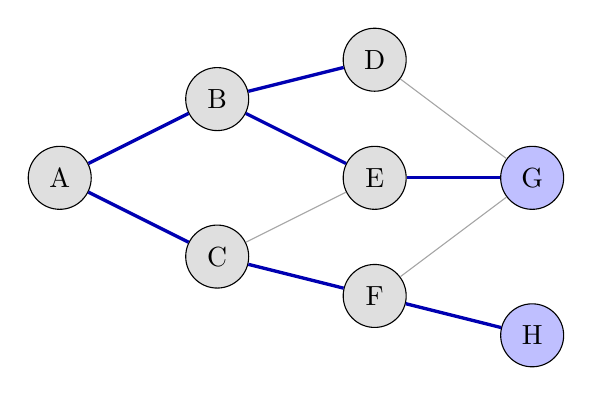
\begin{tikzpicture}[scale=1.0]
  \node[visited] (A) at (0,0) {A};
  \node[visited] (B) at (2,1) {B};
  \node[visited] (C) at (2,-1) {C};
  \node[visited] (D) at (4,1.5) {D};
  \node[visited] (E) at (4,0) {E};
  \node[visited] (F) at (4,-1.5) {F};
  \node[frontier] (G) at (6,0) {G};
  \node[frontier] (H) at (6,-2) {H};

  \draw[treeedge] (A) -- (B);
  \draw[treeedge] (A) -- (C);
  \draw[treeedge] (B) -- (D);
  \draw[treeedge] (B) -- (E);
  \draw[graphedge] (C) -- (E);
  \draw[treeedge] (C) -- (F);
  \draw[graphedge] (D) -- (G);
  \draw[treeedge] (E) -- (G);
  \draw[graphedge] (F) -- (G);
  \draw[treeedge] (F) -- (H);
\end{tikzpicture}
\caption{Passo 3 da BFS: \texttt{G} e \texttt{H} sao descobertos no nivel 3.}
\label{fig:bfs-step3}
\end{figure}

Depois da expansao de \texttt{G}, nenhum novo vertice e encontrado. A proxima
fronteira fica vazia e o algoritmo termina. O resultado e uma arvore de BFS na
qual cada vertice alcancavel possui um pai em um nivel imediatamente anterior ao
seu.

\section{Divisão do Grafo entre Workers}

Em uma implementação paralela ou distribuída, o grafo não precisa ficar inteiro
em um único processo. Uma estratégia comum é dividir seus vértices entre vários
\textit{workers}. Cada worker fica responsável por armazenar e processar uma
parte dos vértices e de suas listas de adjacência. Durante a BFS, quando um
worker expande um vértice local, ele examina suas arestas; se o vizinho pertence
a outro worker, a descoberta desse vizinho precisa ser comunicada ao worker que
o possui.

Uma forma simples de particionamento é a distribuição cíclica. Com quatro
workers, o dono de um vértice pode ser calculado por:

\begin{lstlisting}
worker(v) = v mod 4
\end{lstlisting}

Assim, os vértices são distribuídos de maneira alternada entre os workers. Essa
estratégia não garante balanceamento perfeito para todos os grafos, mas é simples
e evita concentrar intervalos inteiros de vértices em um único worker. A
Tabela~\ref{tab:worker-partition} mostra um exemplo com 16 vértices.

\begin{table}[H]
\centering
\begin{tabular}{c|c}
Worker & Vértices pertencentes ao worker \\
\hline
0 & 0, 4, 8, 12 \\
1 & 1, 5, 9, 13 \\
2 & 2, 6, 10, 14 \\
3 & 3, 7, 11, 15 \\
\end{tabular}
\caption{Particionamento cíclico de 16 vértices entre 4 workers.}
\label{tab:worker-partition}
\end{table}

A Figura~\ref{fig:grafo-global-workers} mostra a visão global de um grafo com 16
vértices. Essa visão representa o grafo completo antes de considerar qual worker
é responsável por cada vértice.

\begin{figure}[H]
\centering
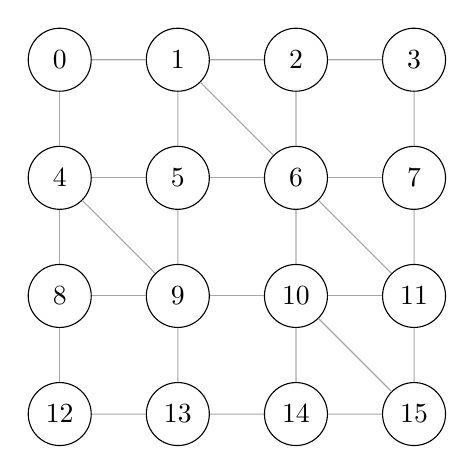
\begin{tikzpicture}[scale=0.75]
  \foreach \i/\x/\y in {0/0/3,1/2/3,2/4/3,3/6/3,
                        4/0/1,5/2/1,6/4/1,7/6/1,
                        8/0/-1,9/2/-1,10/4/-1,11/6/-1,
                        12/0/-3,13/2/-3,14/4/-3,15/6/-3} {
    \node[vertex] (v\i) at (\x,\y) {\i};
  }

  \draw[graphedge] (v0) -- (v1);
  \draw[graphedge] (v1) -- (v2);
  \draw[graphedge] (v2) -- (v3);
  \draw[graphedge] (v0) -- (v4);
  \draw[graphedge] (v1) -- (v5);
  \draw[graphedge] (v2) -- (v6);
  \draw[graphedge] (v3) -- (v7);
  \draw[graphedge] (v4) -- (v5);
  \draw[graphedge] (v5) -- (v6);
  \draw[graphedge] (v6) -- (v7);
  \draw[graphedge] (v4) -- (v8);
  \draw[graphedge] (v5) -- (v9);
  \draw[graphedge] (v6) -- (v10);
  \draw[graphedge] (v7) -- (v11);
  \draw[graphedge] (v8) -- (v9);
  \draw[graphedge] (v9) -- (v10);
  \draw[graphedge] (v10) -- (v11);
  \draw[graphedge] (v8) -- (v12);
  \draw[graphedge] (v9) -- (v13);
  \draw[graphedge] (v10) -- (v14);
  \draw[graphedge] (v11) -- (v15);
  \draw[graphedge] (v12) -- (v13);
  \draw[graphedge] (v13) -- (v14);
  \draw[graphedge] (v14) -- (v15);
  \draw[graphedge] (v1) -- (v6);
  \draw[graphedge] (v4) -- (v9);
  \draw[graphedge] (v6) -- (v11);
  \draw[graphedge] (v10) -- (v15);
\end{tikzpicture}
\caption{Visão global de um grafo com 16 vértices antes do particionamento.}
\label{fig:grafo-global-workers}
\end{figure}

A Figura~\ref{fig:grafo-particionado-workers} mostra o mesmo grafo particionado
entre quatro workers. As cores indicam o dono de cada vértice. As arestas que
ligam vértices de cores diferentes representam comunicações potenciais durante a
BFS, pois a expansão de um vértice em um worker pode descobrir um vértice que
pertence a outro worker.

\begin{figure}[H]
\centering
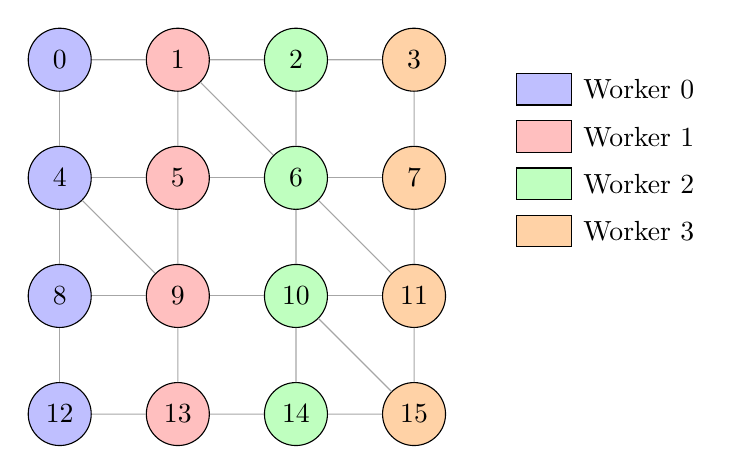
\begin{tikzpicture}[scale=0.75]
  \foreach \i/\x/\y/\c in {0/0/3/blue!25,1/2/3/red!25,2/4/3/green!25,3/6/3/orange!35,
                           4/0/1/blue!25,5/2/1/red!25,6/4/1/green!25,7/6/1/orange!35,
                           8/0/-1/blue!25,9/2/-1/red!25,10/4/-1/green!25,11/6/-1/orange!35,
                           12/0/-3/blue!25,13/2/-3/red!25,14/4/-3/green!25,15/6/-3/orange!35} {
    \node[circle, draw, fill=\c, minimum size=8mm, inner sep=0pt] (p\i) at (\x,\y) {\i};
  }

  \draw[graphedge] (p0) -- (p1);
  \draw[graphedge] (p1) -- (p2);
  \draw[graphedge] (p2) -- (p3);
  \draw[graphedge] (p0) -- (p4);
  \draw[graphedge] (p1) -- (p5);
  \draw[graphedge] (p2) -- (p6);
  \draw[graphedge] (p3) -- (p7);
  \draw[graphedge] (p4) -- (p5);
  \draw[graphedge] (p5) -- (p6);
  \draw[graphedge] (p6) -- (p7);
  \draw[graphedge] (p4) -- (p8);
  \draw[graphedge] (p5) -- (p9);
  \draw[graphedge] (p6) -- (p10);
  \draw[graphedge] (p7) -- (p11);
  \draw[graphedge] (p8) -- (p9);
  \draw[graphedge] (p9) -- (p10);
  \draw[graphedge] (p10) -- (p11);
  \draw[graphedge] (p8) -- (p12);
  \draw[graphedge] (p9) -- (p13);
  \draw[graphedge] (p10) -- (p14);
  \draw[graphedge] (p11) -- (p15);
  \draw[graphedge] (p12) -- (p13);
  \draw[graphedge] (p13) -- (p14);
  \draw[graphedge] (p14) -- (p15);
  \draw[graphedge] (p1) -- (p6);
  \draw[graphedge] (p4) -- (p9);
  \draw[graphedge] (p6) -- (p11);
  \draw[graphedge] (p10) -- (p15);

  \node[draw, fill=blue!25, minimum width=7mm, minimum height=4mm] at (8.2,2.5) {};
  \node[anchor=west] at (8.7,2.5) {Worker 0};
  \node[draw, fill=red!25, minimum width=7mm, minimum height=4mm] at (8.2,1.7) {};
  \node[anchor=west] at (8.7,1.7) {Worker 1};
  \node[draw, fill=green!25, minimum width=7mm, minimum height=4mm] at (8.2,0.9) {};
  \node[anchor=west] at (8.7,0.9) {Worker 2};
  \node[draw, fill=orange!35, minimum width=7mm, minimum height=4mm] at (8.2,0.1) {};
  \node[anchor=west] at (8.7,0.1) {Worker 3};
\end{tikzpicture}
\caption{Mesmo grafo particionado entre 4 workers usando a regra $worker(v) = v \bmod 4$.}
\label{fig:grafo-particionado-workers}
\end{figure}

\subsection{Exemplo de BFS Paralela com 4 Workers}

Considere uma BFS iniciada no vértice 0 do grafo particionado da
Figura~\ref{fig:grafo-particionado-workers}. No passo inicial, apenas o worker 0
possui trabalho, pois ele é o dono do vértice 0. Ao expandir 0, são descobertos
os vértices 1 e 4. O vértice 4 pertence ao próprio worker 0, enquanto o vértice 1
pertence ao worker 1. Portanto, a nova fronteira já fica distribuída entre mais
de um worker.

Após a expansão dos vértices 1 e 4, a BFS chega ao passo mostrado na
Figura~\ref{fig:bfs-paralela-step2}. Nesse momento, a fronteira global de
nível 2 é formada por vértices armazenados em workers diferentes. O worker 0
possui o vértice 8 na fronteira, o worker 1 possui os vértices 5 e 9, o worker 2
possui os vértices 2 e 6, e o worker 3 ainda não possui vértices na fronteira
atual.

A expansão passo a passo é mostrada nas figuras seguintes. Em cada uma delas, a
fronteira global é dividida entre os quatro workers. Os vértices em azul formam
a fronteira local do passo atual, os vértices em cinza já foram visitados, e os
vértices em branco ainda não foram descobertos. Depois que todos os workers
expandem suas fronteiras locais, os vértices recém-descobertos formam a
fronteira do próximo nível.

No passo 0, apenas o worker 0 possui trabalho, pois a origem 0 pertence a ele.

\begin{figure}[H]
\centering
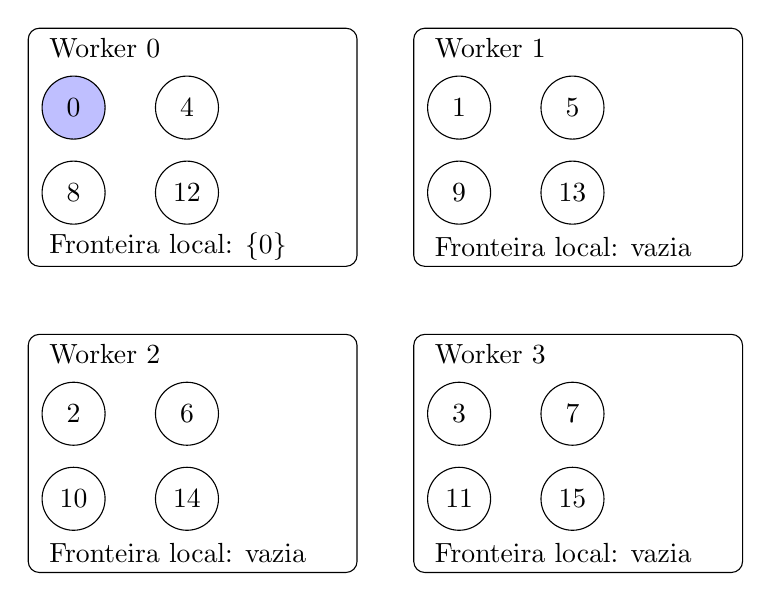
\begin{tikzpicture}[scale=0.72]
  \draw[rounded corners] (-0.8,-0.8) rectangle (5.0,3.4);
  \node[anchor=west] at (-0.6,3.05) {Worker 0};
  \node[frontier] (s0w0v0) at (0,2) {0};
  \node[undiscovered] (s0w0v4) at (2,2) {4};
  \node[undiscovered] (s0w0v8) at (0,0.5) {8};
  \node[undiscovered] (s0w0v12) at (2,0.5) {12};
  \node[anchor=west] at (-0.6,-0.45) {Fronteira local: \{0\}};

  \draw[rounded corners] (6.0,-0.8) rectangle (11.8,3.4);
  \node[anchor=west] at (6.2,3.05) {Worker 1};
  \node[undiscovered] at (6.8,2) {1};
  \node[undiscovered] at (8.8,2) {5};
  \node[undiscovered] at (6.8,0.5) {9};
  \node[undiscovered] at (8.8,0.5) {13};
  \node[anchor=west] at (6.2,-0.45) {Fronteira local: vazia};

  \draw[rounded corners] (-0.8,-6.2) rectangle (5.0,-2.0);
  \node[anchor=west] at (-0.6,-2.35) {Worker 2};
  \node[undiscovered] at (0,-3.4) {2};
  \node[undiscovered] at (2,-3.4) {6};
  \node[undiscovered] at (0,-4.9) {10};
  \node[undiscovered] at (2,-4.9) {14};
  \node[anchor=west] at (-0.6,-5.85) {Fronteira local: vazia};

  \draw[rounded corners] (6.0,-6.2) rectangle (11.8,-2.0);
  \node[anchor=west] at (6.2,-2.35) {Worker 3};
  \node[undiscovered] at (6.8,-3.4) {3};
  \node[undiscovered] at (8.8,-3.4) {7};
  \node[undiscovered] at (6.8,-4.9) {11};
  \node[undiscovered] at (8.8,-4.9) {15};
  \node[anchor=west] at (6.2,-5.85) {Fronteira local: vazia};
\end{tikzpicture}
\caption{Passo 0 da BFS paralela: apenas a origem 0 está na fronteira.}
\label{fig:bfs-paralela-step0}
\end{figure}

Ao expandir 0, são descobertos 1 e 4. O vértice 4 permanece no worker 0, e o
vértice 1 passa a compor a fronteira local do worker 1.

\begin{figure}[H]
\centering
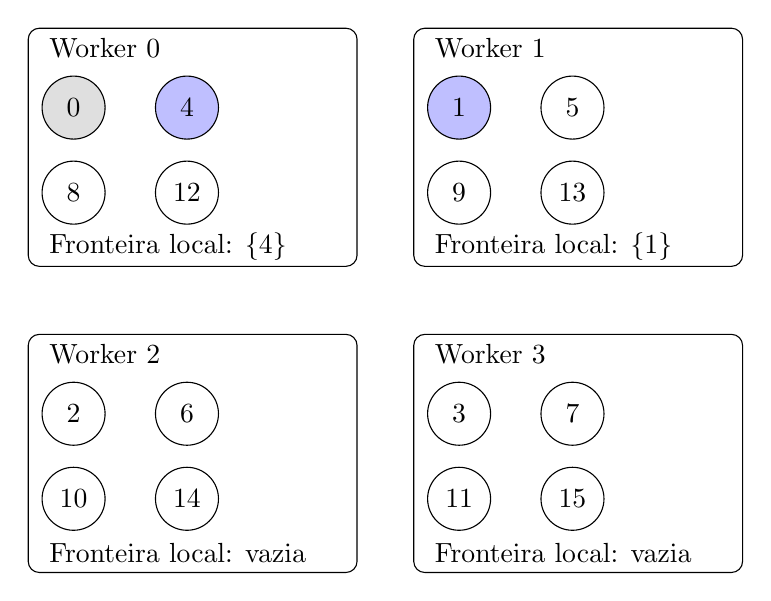
\begin{tikzpicture}[scale=0.72]
  \draw[rounded corners] (-0.8,-0.8) rectangle (5.0,3.4);
  \node[anchor=west] at (-0.6,3.05) {Worker 0};
  \node[visited] at (0,2) {0};
  \node[frontier] at (2,2) {4};
  \node[undiscovered] at (0,0.5) {8};
  \node[undiscovered] at (2,0.5) {12};
  \node[anchor=west] at (-0.6,-0.45) {Fronteira local: \{4\}};

  \draw[rounded corners] (6.0,-0.8) rectangle (11.8,3.4);
  \node[anchor=west] at (6.2,3.05) {Worker 1};
  \node[frontier] at (6.8,2) {1};
  \node[undiscovered] at (8.8,2) {5};
  \node[undiscovered] at (6.8,0.5) {9};
  \node[undiscovered] at (8.8,0.5) {13};
  \node[anchor=west] at (6.2,-0.45) {Fronteira local: \{1\}};

  \draw[rounded corners] (-0.8,-6.2) rectangle (5.0,-2.0);
  \node[anchor=west] at (-0.6,-2.35) {Worker 2};
  \node[undiscovered] at (0,-3.4) {2};
  \node[undiscovered] at (2,-3.4) {6};
  \node[undiscovered] at (0,-4.9) {10};
  \node[undiscovered] at (2,-4.9) {14};
  \node[anchor=west] at (-0.6,-5.85) {Fronteira local: vazia};

  \draw[rounded corners] (6.0,-6.2) rectangle (11.8,-2.0);
  \node[anchor=west] at (6.2,-2.35) {Worker 3};
  \node[undiscovered] at (6.8,-3.4) {3};
  \node[undiscovered] at (8.8,-3.4) {7};
  \node[undiscovered] at (6.8,-4.9) {11};
  \node[undiscovered] at (8.8,-4.9) {15};
  \node[anchor=west] at (6.2,-5.85) {Fronteira local: vazia};
\end{tikzpicture}
\caption{Passo 1 da BFS paralela: os workers 0 e 1 possuem vértices na fronteira.}
\label{fig:bfs-paralela-step1}
\end{figure}

No passo 1, os workers 0 e 1 trabalham ao mesmo tempo: 4 descobre 8 e 9,
enquanto 1 descobre 2, 5 e 6. No passo 2, já há trabalho em três workers
diferentes.

\begin{figure}[H]
\centering
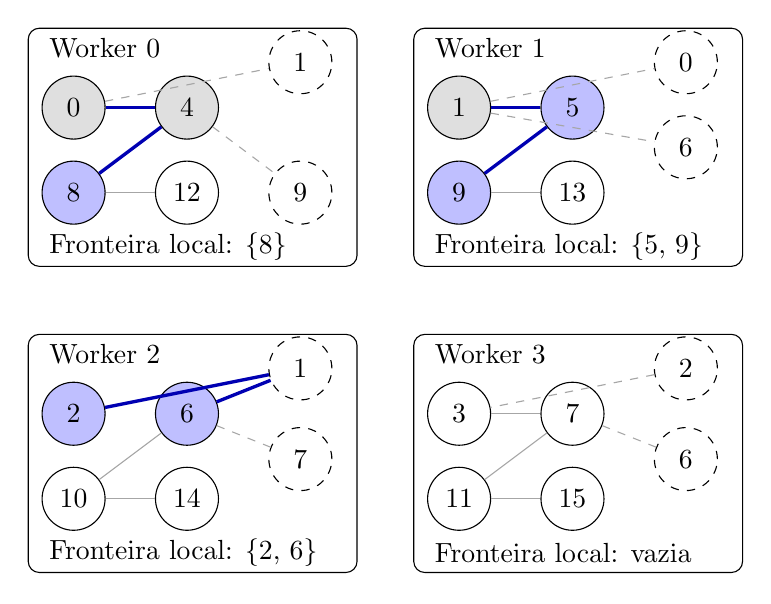
\begin{tikzpicture}[scale=0.72]
  \draw[rounded corners] (-0.8,-0.8) rectangle (5.0,3.4);
  \node[anchor=west] at (-0.6,3.05) {Worker 0};
  \node[visited] (w0v0) at (0,2) {0};
  \node[visited] (w0v4) at (2,2) {4};
  \node[frontier] (w0v8) at (0,0.5) {8};
  \node[undiscovered] (w0v12) at (2,0.5) {12};
  \node[draw, dashed, circle, minimum size=8mm, inner sep=0pt] (w0g1) at (4,2.8) {1};
  \node[draw, dashed, circle, minimum size=8mm, inner sep=0pt] (w0g9) at (4,0.5) {9};
  \draw[treeedge] (w0v0) -- (w0v4);
  \draw[treeedge] (w0v4) -- (w0v8);
  \draw[graphedge] (w0v8) -- (w0v12);
  \draw[graphedge, dashed] (w0v0) -- (w0g1);
  \draw[graphedge, dashed] (w0v4) -- (w0g9);
  \node[anchor=west] at (-0.6,-0.45) {Fronteira local: \{8\}};

  \draw[rounded corners] (6.0,-0.8) rectangle (11.8,3.4);
  \node[anchor=west] at (6.2,3.05) {Worker 1};
  \node[visited] (w1v1) at (6.8,2) {1};
  \node[frontier] (w1v5) at (8.8,2) {5};
  \node[frontier] (w1v9) at (6.8,0.5) {9};
  \node[undiscovered] (w1v13) at (8.8,0.5) {13};
  \node[draw, dashed, circle, minimum size=8mm, inner sep=0pt] (w1g0) at (10.8,2.8) {0};
  \node[draw, dashed, circle, minimum size=8mm, inner sep=0pt] (w1g6) at (10.8,1.3) {6};
  \draw[treeedge] (w1v1) -- (w1v5);
  \draw[treeedge] (w1v5) -- (w1v9);
  \draw[graphedge] (w1v9) -- (w1v13);
  \draw[graphedge, dashed] (w1v1) -- (w1g0);
  \draw[graphedge, dashed] (w1v1) -- (w1g6);
  \node[anchor=west] at (6.2,-0.45) {Fronteira local: \{5, 9\}};

  \draw[rounded corners] (-0.8,-6.2) rectangle (5.0,-2.0);
  \node[anchor=west] at (-0.6,-2.35) {Worker 2};
  \node[frontier] (w2v2) at (0,-3.4) {2};
  \node[frontier] (w2v6) at (2,-3.4) {6};
  \node[undiscovered] (w2v10) at (0,-4.9) {10};
  \node[undiscovered] (w2v14) at (2,-4.9) {14};
  \node[draw, dashed, circle, minimum size=8mm, inner sep=0pt] (w2g1) at (4,-2.6) {1};
  \node[draw, dashed, circle, minimum size=8mm, inner sep=0pt] (w2g7) at (4,-4.2) {7};
  \draw[treeedge] (w2g1) -- (w2v2);
  \draw[treeedge] (w2g1) -- (w2v6);
  \draw[graphedge] (w2v6) -- (w2v10);
  \draw[graphedge] (w2v10) -- (w2v14);
  \draw[graphedge, dashed] (w2v6) -- (w2g7);
  \node[anchor=west] at (-0.6,-5.85) {Fronteira local: \{2, 6\}};

  \draw[rounded corners] (6.0,-6.2) rectangle (11.8,-2.0);
  \node[anchor=west] at (6.2,-2.35) {Worker 3};
  \node[undiscovered] (w3v3) at (6.8,-3.4) {3};
  \node[undiscovered] (w3v7) at (8.8,-3.4) {7};
  \node[undiscovered] (w3v11) at (6.8,-4.9) {11};
  \node[undiscovered] (w3v15) at (8.8,-4.9) {15};
  \node[draw, dashed, circle, minimum size=8mm, inner sep=0pt] (w3g2) at (10.8,-2.6) {2};
  \node[draw, dashed, circle, minimum size=8mm, inner sep=0pt] (w3g6) at (10.8,-4.2) {6};
  \draw[graphedge] (w3v3) -- (w3v7);
  \draw[graphedge] (w3v7) -- (w3v11);
  \draw[graphedge] (w3v11) -- (w3v15);
  \draw[graphedge, dashed] (w3g2) -- (w3v3);
  \draw[graphedge, dashed] (w3g6) -- (w3v7);
  \node[anchor=west] at (6.2,-5.85) {Fronteira local: vazia};
\end{tikzpicture}
\caption{Passo 2 da BFS paralela: a fronteira global está distribuída entre os workers 0, 1 e 2. Vértices tracejados representam vizinhos remotos mantidos apenas para ilustrar comunicações entre workers.}
\label{fig:bfs-paralela-step2}
\end{figure}

No passo 2, a expansão dos vértices 2 e 6 no worker 2 gera trabalho para o
worker 3, pois existem arestas para os vértices 3 e 7. Ao mesmo tempo, os workers
0, 1 e 2 descobrem outros vértices locais, formando a próxima fronteira.

\begin{figure}[H]
\centering
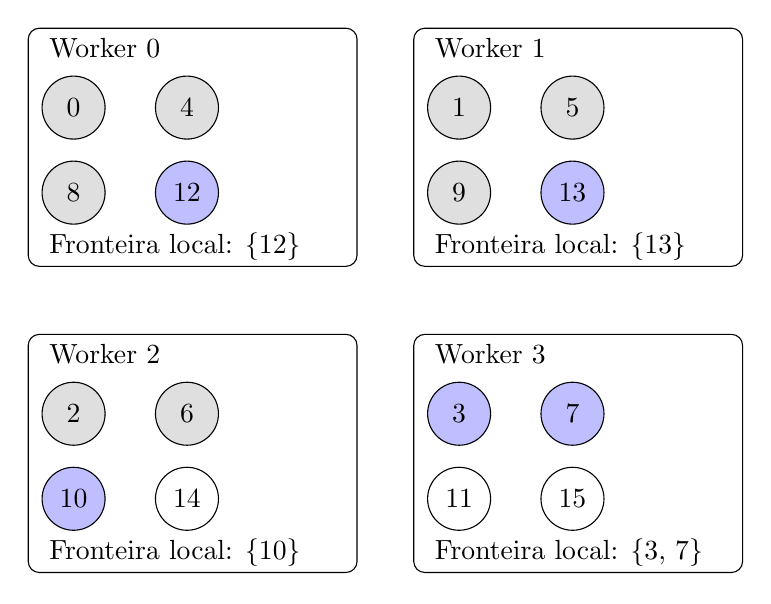
\begin{tikzpicture}[scale=0.72]
  \draw[rounded corners] (-0.8,-0.8) rectangle (5.0,3.4);
  \node[anchor=west] at (-0.6,3.05) {Worker 0};
  \node[visited] at (0,2) {0};
  \node[visited] at (2,2) {4};
  \node[visited] at (0,0.5) {8};
  \node[frontier] at (2,0.5) {12};
  \node[anchor=west] at (-0.6,-0.45) {Fronteira local: \{12\}};

  \draw[rounded corners] (6.0,-0.8) rectangle (11.8,3.4);
  \node[anchor=west] at (6.2,3.05) {Worker 1};
  \node[visited] at (6.8,2) {1};
  \node[visited] at (8.8,2) {5};
  \node[visited] at (6.8,0.5) {9};
  \node[frontier] at (8.8,0.5) {13};
  \node[anchor=west] at (6.2,-0.45) {Fronteira local: \{13\}};

  \draw[rounded corners] (-0.8,-6.2) rectangle (5.0,-2.0);
  \node[anchor=west] at (-0.6,-2.35) {Worker 2};
  \node[visited] at (0,-3.4) {2};
  \node[visited] at (2,-3.4) {6};
  \node[frontier] at (0,-4.9) {10};
  \node[undiscovered] at (2,-4.9) {14};
  \node[anchor=west] at (-0.6,-5.85) {Fronteira local: \{10\}};

  \draw[rounded corners] (6.0,-6.2) rectangle (11.8,-2.0);
  \node[anchor=west] at (6.2,-2.35) {Worker 3};
  \node[frontier] at (6.8,-3.4) {3};
  \node[frontier] at (8.8,-3.4) {7};
  \node[undiscovered] at (6.8,-4.9) {11};
  \node[undiscovered] at (8.8,-4.9) {15};
  \node[anchor=west] at (6.2,-5.85) {Fronteira local: \{3, 7\}};
\end{tikzpicture}
\caption{Passo 3 da BFS paralela: todos os workers possuem vértices na fronteira.}
\label{fig:bfs-paralela-step3}
\end{figure}

Após o passo 3, apenas os workers 2 e 3 continuam com novos vértices a expandir.

\begin{figure}[H]
\centering
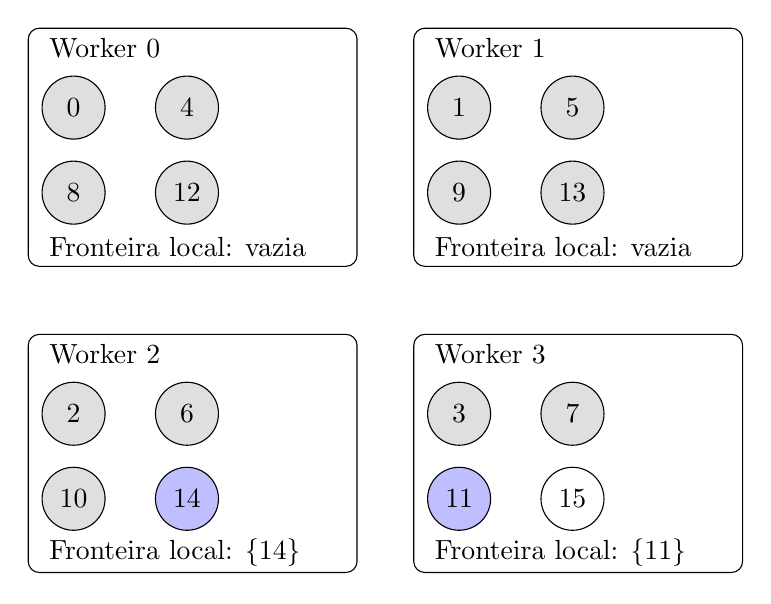
\begin{tikzpicture}[scale=0.72]
  \draw[rounded corners] (-0.8,-0.8) rectangle (5.0,3.4);
  \node[anchor=west] at (-0.6,3.05) {Worker 0};
  \node[visited] at (0,2) {0};
  \node[visited] at (2,2) {4};
  \node[visited] at (0,0.5) {8};
  \node[visited] at (2,0.5) {12};
  \node[anchor=west] at (-0.6,-0.45) {Fronteira local: vazia};

  \draw[rounded corners] (6.0,-0.8) rectangle (11.8,3.4);
  \node[anchor=west] at (6.2,3.05) {Worker 1};
  \node[visited] at (6.8,2) {1};
  \node[visited] at (8.8,2) {5};
  \node[visited] at (6.8,0.5) {9};
  \node[visited] at (8.8,0.5) {13};
  \node[anchor=west] at (6.2,-0.45) {Fronteira local: vazia};

  \draw[rounded corners] (-0.8,-6.2) rectangle (5.0,-2.0);
  \node[anchor=west] at (-0.6,-2.35) {Worker 2};
  \node[visited] at (0,-3.4) {2};
  \node[visited] at (2,-3.4) {6};
  \node[visited] at (0,-4.9) {10};
  \node[frontier] at (2,-4.9) {14};
  \node[anchor=west] at (-0.6,-5.85) {Fronteira local: \{14\}};

  \draw[rounded corners] (6.0,-6.2) rectangle (11.8,-2.0);
  \node[anchor=west] at (6.2,-2.35) {Worker 3};
  \node[visited] at (6.8,-3.4) {3};
  \node[visited] at (8.8,-3.4) {7};
  \node[frontier] at (6.8,-4.9) {11};
  \node[undiscovered] at (8.8,-4.9) {15};
  \node[anchor=west] at (6.2,-5.85) {Fronteira local: \{11\}};
\end{tikzpicture}
\caption{Passo 4 da BFS paralela: apenas os workers 2 e 3 continuam com fronteiras locais.}
\label{fig:bfs-paralela-step4}
\end{figure}

Por fim, a expansão de 11 ou 14 descobre 15, que pertence ao worker 3. Depois de
expandir 15, nenhuma nova descoberta é produzida e a BFS termina.

\begin{figure}[H]
\centering
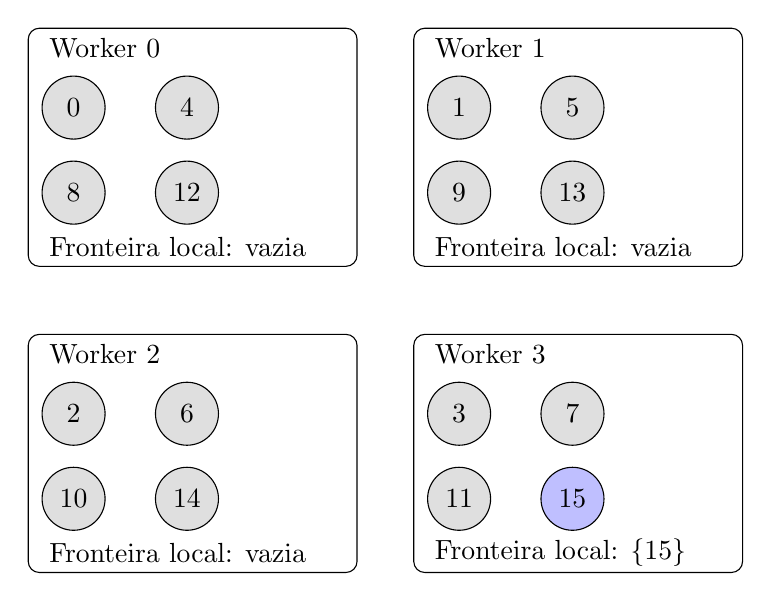
\begin{tikzpicture}[scale=0.72]
  \draw[rounded corners] (-0.8,-0.8) rectangle (5.0,3.4);
  \node[anchor=west] at (-0.6,3.05) {Worker 0};
  \node[visited] at (0,2) {0};
  \node[visited] at (2,2) {4};
  \node[visited] at (0,0.5) {8};
  \node[visited] at (2,0.5) {12};
  \node[anchor=west] at (-0.6,-0.45) {Fronteira local: vazia};

  \draw[rounded corners] (6.0,-0.8) rectangle (11.8,3.4);
  \node[anchor=west] at (6.2,3.05) {Worker 1};
  \node[visited] at (6.8,2) {1};
  \node[visited] at (8.8,2) {5};
  \node[visited] at (6.8,0.5) {9};
  \node[visited] at (8.8,0.5) {13};
  \node[anchor=west] at (6.2,-0.45) {Fronteira local: vazia};

  \draw[rounded corners] (-0.8,-6.2) rectangle (5.0,-2.0);
  \node[anchor=west] at (-0.6,-2.35) {Worker 2};
  \node[visited] at (0,-3.4) {2};
  \node[visited] at (2,-3.4) {6};
  \node[visited] at (0,-4.9) {10};
  \node[visited] at (2,-4.9) {14};
  \node[anchor=west] at (-0.6,-5.85) {Fronteira local: vazia};

  \draw[rounded corners] (6.0,-6.2) rectangle (11.8,-2.0);
  \node[anchor=west] at (6.2,-2.35) {Worker 3};
  \node[visited] at (6.8,-3.4) {3};
  \node[visited] at (8.8,-3.4) {7};
  \node[visited] at (6.8,-4.9) {11};
  \node[frontier] at (8.8,-4.9) {15};
  \node[anchor=west] at (6.2,-5.85) {Fronteira local: \{15\}};
\end{tikzpicture}
\caption{Passo 5 da BFS paralela: o último vértice da fronteira está no worker 3.}
\label{fig:bfs-paralela-step5}
\end{figure}

Essa sequência visual mostra que a fronteira global da BFS é a união das
fronteiras locais de cada worker. Em uma implementação paralela, cada worker
expande apenas os vértices da sua fronteira local. Quando uma aresta aponta para
um vértice remoto, a atualização precisa ser enviada ao worker dono daquele
vértice, que poderá processá-lo no próximo passo.

\section{Problemas Reais}

Grafos aparecem naturalmente em problemas reais de grande escala. Em uma rede
social, vertices podem representar usuarios e arestas podem representar
amizades, seguidores, mensagens ou interacoes \cite{easleykleinberg}. Na Web,
paginas sao vertices e hiperlinks sao arestas \cite{brinpage}. Em seguranca
computacional, grafos podem modelar fluxos de rede, dependencias entre
processos, tentativas de acesso e relacoes entre entidades suspeitas
\cite{akoglugraphanomaly}. Em biologia, vertices podem representar proteinas,
genes ou moléculas, e arestas podem representar interacoes
\cite{barabasinetworkbiology}. Em todos esses casos, a BFS aparece como uma
primitiva para calcular alcancabilidade, distancia em numero de arestas e
expansao de vizinhanca.

A literatura de sistemas de grafos trata a BFS como uma das operacoes centrais
para avaliar plataformas de processamento de dados irregulares. O Graph500 foi
proposto para complementar benchmarks numericos tradicionais com uma carga de
trabalho orientada a dados, motivado pela diferenca entre simulacoes fisicas,
que tendem a ser estruturadas e intensivas em ponto flutuante, e aplicacoes de
informatica, que tendem a ser nao estruturadas, orientadas a inteiros e com
baixa localidade \cite{murphygraph500}. Sua especificacao define a BFS como o
Kernel 2 do benchmark, executado sobre grafos sinteticos de escala crescente, e
usa a metrica TEPS, ou arestas atravessadas por segundo, para medir desempenho
\cite{graph500spec}. Isso mostra que a BFS nao e apenas um exercicio teorico:
ela e usada como proxy para medir a capacidade de supercomputadores processarem
analise de grafos massivos.

Em redes sociais, a BFS modela consultas de vizinhanca e distancia social. A
pergunta ``quais usuarios estao a ate dois ou tres saltos de uma conta?'' e uma
execucao limitada de BFS. Esse tipo de consulta aparece em recomendacao de
amizades, propagacao de informacao, deteccao de comunidades locais e analise de
influencia \cite{easleykleinberg}. Em grafos com bilhoes de relacoes, a
expansao de poucos niveis pode atingir uma quantidade enorme de vertices,
especialmente quando existem hubs de grau muito alto. Por isso, mesmo uma BFS
limitada por profundidade pode exigir processamento paralelo e estruturas de
dados distribuidas.

Em grafos da Web, a BFS tambem e uma abstracao natural. Um rastreador
\textit{web crawler} pode iniciar em um conjunto de paginas sementes e expandir
links por camadas, descobrindo novas paginas a cada nivel \cite{brinpage}. O
sistema Pregel, do Google, foi proposto para processamento de grafos em larga
escala e apresenta algoritmos como caminhos minimos, PageRank, propagacao de
rotulos e outras computacoes iterativas sobre grafos distribuidos \cite{pregel}.
Embora Pregel seja um modelo mais geral que BFS, sua execucao em superpassos e
troca de mensagens entre vertices e muito proxima da ideia de fronteiras
sucessivas usada em BFS distribuida.

Em seguranca, investigacao de fraudes e analise de dependencias, BFS e usada
para expandir a vizinhanca de uma entidade de interesse. A partir de uma conta,
um endereco IP, uma maquina infectada ou um processo suspeito, a busca em
largura identifica entidades conectadas por poucos saltos. Essa forma de
exploracao e importante porque muitas relacoes relevantes nao aparecem em uma
aresta direta, mas em cadeias curtas: contas que compartilham dispositivos,
maquinas que se comunicam com o mesmo servidor, ou processos que dependem dos
mesmos arquivos \cite{akoglugraphanomaly}. Em grafos corporativos ou de
telecomunicacoes, essas buscas podem envolver centenas de milhoes de vertices e
precisam responder em tempo interativo ou quase interativo.

O desafio e que os grafos modernos podem ser massivos e irregulares. Grafos de
redes sociais e da Web frequentemente possuem distribuicao de grau altamente
desbalanceada: poucos vertices concentram muitas arestas, enquanto a maioria tem
grau baixo. Essa propriedade gera duas dificuldades para BFS. Primeiro, ha
desbalanceamento de trabalho, pois expandir um vertice de alto grau custa muito
mais do que expandir um vertice comum. Segundo, ha muita contencao, pois muitos
caminhos podem tentar descobrir o mesmo vertice ao mesmo tempo.

Alem disso, a BFS tem baixa localidade de memoria. Em matrizes densas ou
vetores, os acessos costumam ser contiguos e previsiveis. Em grafos, ao
expandir a fronteira, o algoritmo segue listas de adjacencia que podem apontar
para posicoes distantes e aparentemente aleatorias. Consequentemente, a BFS e
normalmente limitada por largura de banda, latencia de memoria, atomicos,
sincronizacao e comunicacao entre maquinas, e nao por operacoes aritmeticas.

Trabalhos em arquiteturas paralelas mostram como essas dificuldades aparecem na
pratica. Beamer, Asanovic e Patterson propuseram a BFS \textit{direction
optimizing}, que alterna entre uma expansao top-down, baseada na fronteira
atual, e uma expansao bottom-up, que examina vertices ainda nao visitados
procurando vizinhos na fronteira \cite{beamerbfs}. Essa mudanca reduz trabalho
em grafos de pequeno diametro e grande fronteira, um caso comum em grafos
sociais e da Web. Merrill, Garland e Grimshaw estudaram BFS em GPU e mostraram
que a primitiva e representativa de computacoes paralelas com acesso a memoria e
distribuicao de trabalho irregulares; sua implementacao alcançou bilhoes de
arestas atravessadas por segundo em uma ou mais GPUs \cite{merrillgpu}.

Portanto, BFS aparece em problemas reais de duas formas complementares. Como
algoritmo final, ela responde consultas de alcance, distancia e vizinhanca. Como
primitiva de sistema, ela estressa exatamente os componentes que tornam grafos
massivos dificeis: memoria irregular, fronteiras dinamicas, atomicos,
desbalanceamento e comunicacao. Por isso, estudar BFS em GPU e em ambientes
distribuidos e uma forma direta de estudar o desempenho de analise de grafos em
escala real.

\section{Motivacao de Paralelismo}

A BFS possui uma oportunidade natural de paralelismo: todos os vertices de uma
mesma fronteira podem ser processados simultaneamente. Como eles pertencem ao
mesmo nivel da busca, a expansao de suas arestas pode ocorrer em paralelo desde
que a implementacao controle corretamente a descoberta de vertices repetidos.
Se dois ou mais trabalhadores encontram o mesmo vizinho ao mesmo tempo, apenas
um deles deve registrar esse vertice como descoberto e inseri-lo na proxima
fronteira.

Essa propriedade torna a BFS adequada para GPUs, que sao projetadas para
executar milhares de threads leves em paralelo. Em uma GPU, diferentes threads
podem examinar vertices ou arestas distintas da fronteira. Quando a fronteira e
grande, o algoritmo pode expor paralelismo suficiente para ocupar muitos
multiprocessadores da GPU. Como a BFS realiza pouca computacao por aresta, o
principal ganho esperado vem da capacidade da GPU de sustentar muitas operacoes
de memoria simultaneas e esconder parte da latencia por meio de concorrencia.

No entanto, paralelizar BFS em GPU nao e trivial. A primeira dificuldade e o
desbalanceamento de carga. Em grafos com distribuicao de grau irregular, uma
thread responsavel por um vertice de grau muito alto pode ter muito mais
trabalho do que outra thread responsavel por um vertice de grau baixo. Por
isso, implementacoes eficientes geralmente distribuem o trabalho por arestas,
por grupos de threads ou por blocos, em vez de usar sempre uma thread por
vertice.

A segunda dificuldade e a construcao da proxima fronteira. Muitos threads podem
descobrir novos vertices ao mesmo tempo, entao a estrutura que armazena a
fronteira precisa aceitar insercoes concorrentes. Isso normalmente exige
operacoes atomicas, como incremento atomico de um contador de tamanho ou
compare-and-swap no vetor de pais. Essas operacoes garantem corretude, mas
podem causar contencao quando muitas threads tentam atualizar a mesma regiao de
memoria.

A terceira dificuldade aparece em ambientes distribuidos. Quando o grafo nao
cabe em uma unica GPU, vertices e arestas precisam ser particionados entre
varios processos ou dispositivos. Durante a expansao da fronteira, uma aresta
pode apontar para um vertice pertencente a outro processo. Nesse caso, a
descoberta precisa ser comunicada ao proprietario do vertice remoto. Como o
padrao de comunicacao depende dos dados do grafo e muda a cada nivel da BFS,
essa comunicacao e irregular e dificil de otimizar com mensagens grandes e
previsiveis.

Portanto, a motivacao para usar paralelismo em GPU e dupla. Primeiro, a BFS
precisa de alto paralelismo para processar grandes volumes de arestas em tempo
razoavel. Segundo, sistemas modernos de GPU oferecem alta largura de banda de
memoria e interconexoes rapidas entre dispositivos, caracteristicas importantes
para algoritmos de grafos massivos. O desafio de pesquisa e organizar o trabalho
e a comunicacao de forma alinhada ao hardware.

\section{Implementacao GPU side em NVSHMEM}

NVSHMEM e uma biblioteca de comunicacao para GPUs baseada no modelo de espaco
de enderecamento global particionado. Nesse modelo, cada elemento de
processamento, ou PE, possui sua memoria local, mas tambem pode acessar regioes
simetricas de memoria de outros PEs por meio de operacoes de comunicacao
unilaterais. A diferenca importante para este trabalho e que essas operacoes
podem ser chamadas diretamente de kernels CUDA, isto e, pelo proprio codigo que
esta executando na GPU.

Em uma BFS distribuida, essa capacidade e relevante porque a comunicacao remota
e descoberta dinamicamente. Ao processar uma aresta \texttt{(u, v)}, uma thread
da GPU pode determinar que \texttt{v} pertence a outro PE. Com NVSHMEM, essa
thread pode tentar atualizar diretamente o estado remoto de \texttt{v}, sem
precisar retornar ao CPU para empacotar uma mensagem MPI naquele momento. Isso
reduz a dependencia de comunicacao mediada pelo host e aproxima o mecanismo de
comunicacao do ponto onde a informacao e produzida.

Uma estrategia comum e particionar os vertices de forma ciclica entre os PEs. O
proprietario de um vertice \texttt{v} pode ser calculado como \texttt{v \%
num\_pes}, e o indice local como \texttt{v / num\_pes}. Assim, qualquer thread
consegue descobrir rapidamente qual PE e responsavel por armazenar o estado de
um vertice. O vetor de pais, o vetor de distancias e as estruturas de fronteira
podem ser alocados em memoria simetrica, permitindo atualizacoes locais ou
remotas por NVSHMEM.

O passo principal da BFS em GPU consiste em expandir a fronteira atual. Cada
thread examina uma parte das arestas dos vertices ativos. Para cada vizinho, a
thread verifica se ele ainda nao foi descoberto. Em uma implementacao
concorrente, essa verificacao precisa ser atomica. Um compare-and-swap sobre o
vetor de pais pode trocar o valor inicial, por exemplo \texttt{-1}, pelo pai
que descobriu o vertice. Se a troca for bem-sucedida, a thread sabe que foi a
primeira a descobrir aquele vertice e pode inserir o vizinho na proxima
fronteira.

Quando o vizinho pertence ao mesmo PE, a operacao atomica pode ser local.
Quando pertence a outro PE, a mesma ideia pode ser expressa como uma operacao
atomica remota em NVSHMEM. A operacao remota tenta reivindicar o vertice no PE
proprietario. Esse padrao e adequado para BFS porque a competicao entre varias
descobertas do mesmo vertice e uma corrida benigna: nao e necessario que o
primeiro thread em tempo real seja o pai definitivo, apenas que o pai escolhido
esteja no nivel anterior e que a arvore resultante seja valida.

Um esboco de expansao de fronteira com comunicacao do lado da GPU e mostrado a
seguir:

\begin{lstlisting}
for each active vertex u in current_frontier, in parallel:
    for each neighbor v of u:
        owner = v % num_pes
        local_index = v / num_pes

        old = atomic_compare_and_swap(parent[owner][local_index], -1, u)
        if old == -1:
            insert v into next_frontier of owner
\end{lstlisting}

Na pratica, a implementacao precisa tratar detalhes adicionais. A insercao na
proxima fronteira pode exigir contadores atomicos locais ou remotos. Tambem e
necessario sincronizar os PEs entre niveis para garantir que todas as
descobertas do nivel atual foram completadas antes do inicio do proximo nivel.
Ao final, a BFS termina quando todas as fronteiras locais estao vazias e nenhum
PE possui trabalho pendente.

O uso de NVSHMEM se alinha bem ao comportamento irregular da BFS. Em vez de
forcar a GPU a acumular descobertas, sincronizar com o CPU e entao realizar uma
troca de mensagens, a propria thread que encontra uma aresta remota pode emitir
a atualizacao. Esse modelo nao elimina os custos de comunicacao, atomicos e
sincronizacao, mas reduz a distancia entre computacao e comunicacao. Para
grafos massivos, onde a quantidade de arestas visitadas e grande e o padrao de
destinos e imprevisivel, essa aproximacao pode melhorar a escalabilidade e a
utilizacao do hardware.

No contexto desta tese, a BFS em NVSHMEM representa uma abordagem
\textit{GPU-side}: o CPU continua importante para inicializacao, lancamento dos
processos, configuracao MPI/NVSHMEM e validacao, mas o laco principal de
traversal e comunicacao fina ocorre dentro da GPU. Essa separacao permite usar
MPI para coordenacao global e NVSHMEM para atualizacoes remotas de baixa
granularidade, combinando dois modelos de programacao adequados a camadas
diferentes do sistema.

\bibliographystyle{plain}
\bibliography{bibliografia}

\end{document}
